\documentclass{article}
\usepackage[utf8]{inputenc}
\usepackage{listings}
\usepackage[pdftex]{graphicx}
\usepackage[margin=1in]{geometry}

\title{Udacity Manipulator Arm Report}
\author{Ussama Naal}
\date{May 2019\\v2.0}
\begin{document}

\maketitle

\section{Introduction}

This write-up describes the steps taken to train a Robot Arm Manipulator to grab a static object using DQN techniques. We start first by describing the implementation and changes to the supplied code, then we list the current configuration of  parameters used during training. Finally, we present the results and closing statements.

\section{Implementation}

\subsection{Subscribe to camera and collision topics}

\begin{lstlisting}
void ArmPlugin::Load(physics::ModelPtr _parent, sdf::ElementPtr /*_sdf*/)
{
    ...
    cameraSub = cameraNode->Subscribe(
        "/gazebo/arm\_world/camera/link/camera/image",
        &ArmPlugin::onCameraMsg, this);
    ...
    collisionSub = collisionNode->Subscribe(
        "/gazebo/arm_world/tube/tube_link/my_contact",
        &ArmPlugin::onCollisionMsg, this);
    ...
}
\end{lstlisting}

First line gives us camera feed which is then passed to the deep neural network to process. Second line subscribes to arm contact or collision topic.



\subsection{Create the DQN Agent}

The following code snippet creates the dqnAgent:

\begin{lstlisting}
bool ArmPlugin::createAgent()
{
    ...
    agent = dqnAgent::Create(
        INPUT_WIDTH, INPUT_HEIGHT, INPUT_CHANNELS,
    	DOF * 2, OPTIMIZER, LEARNING_RATE, REPLAY_MEMORY, BATCH_SIZE,
    	GAMMA,
    	EPS_START, EPS_END, EPS_DECAY, USE_LSTM, LSTM_SIZE,
    	ALLOW_RANDOM, DEBUG_DQN );
    ...
}
\end{lstlisting}

\subsection{Velocity or position based control of arm joints}
Within the  ArmPlugin::updateAgent() method, we have the choice to control arm joints through velocity or by adjusting the position.

The following two listing shows the changes made to the code, based on whether the action value is odd or even we decide if the velocity or position change positive or negative. Additionally, I modified the code such that the new velocity or joint deltas updates previous state as increments or decrements.


\begin{lstlisting}
bool ArmPlugin::updateAgent()
{
#if VELOCITY_CONTROL
    ...
    float velocity = actionVelDelta * (action % 2 == 0 ? 1 : -1);
    ...
    vel[action/2] += velocity;  // This was originally a direct assignment
    ...
#else
    ...
    float joint = actionJointDelta * (action % 2 == 0 ? 1 : -1);
    ...
    ref[action/2] += joint; // This was originally a direct assignment 
    ...
#endif
}
\end{lstlisting}

\subsection{Reward for robot gripper hitting the ground}

First I start by impelementing a helper function for checking that whether the gripper hit the or not. The function accepts two parameters, first a bounding box describing the gripper, the other is merely floor level.
\begin{lstlisting}
bool ArmPlugin::checkGroundContact(const math::Box& box, float floor) const
{
	return (box.min.z < floor);
}
\end{lstlisting}

We call this method within ArmPlugin::OnUpdate and if the condition is met we punish the robot with a negative rewards and start a new episode as shown below 
\begin{lstlisting}
void ArmPlugin::OnUpdate(const common::UpdateInfo& updateInfo)
{
	...
	if(checkGroundContact(gripBBox, groundContact))
	{
		if(true){printf("GROUND CONTACT, EOE .................\n");}
		rewardHistory = REWARD_LOSS;
		newReward     = true;
		endEpisode    = true;
	}
	...
}
\end{lstlisting}

\subsection{Issue an interim reward based on the distance to the object}
In this task we need to issue an appropriate reward to the robot as the arm gripper approaches the object. However, we shouldn't rely on the direct changes of distance as they are too noisey. Instead we compute a moving average of the changes. For that we start by declaring a circular buffer to hold the last 5 distance deltas to the object in the ArmPlugin object as follows:
\begin{lstlisting}
class ArmPlugin : public ModelPlugin
    ...
    boost::circular_buffer<float> distDeltas;
\end{lstlisting}

Within ArmPlugin::OnUpdate method, we compute the distnce between the gripper and the arm gripper and the object using the supplied BoxDistance method. We compute the difference from last distance and push the value to the distDeltas buffer and compute the average of the last 5 samples and store in avgGoalDelta. We set the reward by multiplying avgGoalDelta by our defined REWARD\_WIN constant. Details shown in the following listing:

\begin{lstlisting}
void ArmPlugin::OnUpdate(const common::UpdateInfo& updateInfo)
{
	...
    if(!checkGroundContact(gripBBox, groundContact))
    {
        const float distGoal =
            BoxDistance(gripBBox, prop->model->GetBoundingBox());

        if( episodeFrames > 1 )
        {
            const float distDelta  = lastGoalDistance - distGoal;
			
            // compute the smoothed moving average of the delta
            // of the distance to the goal
            distDeltas.push_back(distDelta);
            avgGoalDelta = 0;
            for (auto e : distDeltas)
                avgGoalDelta += e;
            avgGoalDelta /= distDeltas.size();
			
            rewardHistory = avgGoalDelta * REWARD_WIN;
            newReward     = true;
        }

        lastGoalDistance = distGoal;
    }
	...
}
\end{lstlisting}

\subsection{Issue a reward based on collision between the arm’s gripper base and the object}

Earlier we subscribed to the "/gazebo/arm\_world/tube/tube\_link/my\_contact" topic, which notifies us when a contact happen between the arm and another object. We a collision detected we check if the contact between the gripper and the object. If it is the case we issue a reward equivalent to REWARD\_WIN constant and consider the episode done. Otherwise, if the contact was between another part of the arm and the object we issue a loss reward REWARD\_LOSS and consider the episode done too. We consider the later case a loss and terminate the episode since the interaction between the arm body and the object results of the object being pushed away from its place.

\begin{lstlisting}
void ArmPlugin::onCollisionMsg(ConstContactsPtr &contacts)
{
    ...
    successfulTouch = true; /* NEW VARIABLE */

    if (contacts->contact(i).collision1() == COLLISION_ITEM &&
			contacts->contact(i).collision2() == COLLISION_POINT)
    {
        rewardHistory = REWARD_WIN;
        newReward  = true;
        endEpisode = true;
        return;
    }
    else
    {
        rewardHistory = REWARD_LOSS;
        newReward  = true;
        endEpisode = true;
    }
    ...
}
\end{lstlisting}

\subsection{Track the number of successful touches}
The ArmPlugin code already tracks the number of successful grabs, i.e when the target object is touched by the gripper. However, it doesn't track the number of successful touches i.e when the target object is touched by any part of the arm (collision2, gripper, ..). For that we add a new variable named successfulTouches and track and report its value on the console as follows:

\begin{lstlisting}
void ArmPlugin::OnUpdate(const common::UpdateInfo& updateInfo)
{
...
    if (successfulTouch)
    {
    	successfulTouches++;
    	successfulTouch = false;	//reset
    }
    
    printf("Current Accuracy:  "
        "Touches = %0.4f (%03u of %03u), Grabs = %0.4f (%03u of %03u)"
        "(reward=%+0.2f %s)\n",
    	float(successfulTouches)/float(totalRuns), successfulTouches, totalRuns,
    	float(successfulGrabs)/float(totalRuns), successfulGrabs, totalRuns,
    	rewardHistory, (rewardHistory >= REWARD_WIN ? "WIN" : "LOSS"));
...
}
\end{lstlisting}

\section{Tuning}

Table 1, lists all used parameters and their values with a brief explanation to the used values when a value has been changed.

\begin{table}[ht]
\caption{Parameters}
\label{table_example}
\begin{center}
\begin{tabular}{|c||c||c|}
\hline
Parameter & Value & Explanation\\
\hline
VELOCITY\_CONTROL & false & Based on recommendations from one of the mentors \\
\hline
EPS\_START & 0.9f & Default \\
\hline
EPS\_END & 0.05f & Default \\
\hline
EPS\_DECAY & 200 & Default \\
\hline
INPUT\_WIDTH & 64 & Reduced from 512 since gazebo camera output is only 64x64 \\
\hline
INPUT\_HEIGHT & 64 & Reduced from 512 since gazebo camera output is only 64x64 \\
\hline
OPTIMIZER & "RMSprop" & Possibly the only available option \\
\hline
LEARNING\_RATE & 0.1 & With few test this value seems reasonable \\
\hline
REPLAY\_MEMORY & 10000 & Default \\
\hline
BATCH\_SIZE & 64 & Increased from 8: produces more more consistent results \\
\hline
USE\_LSTM & false & true value didn't produce good results for me (see below) \\
\hline
LSTM\_SIZE & 32 & Default: LSTM is not enabled so it doesn't matter \\
\hline
REWARD\_WIN  & 200.0f & Needs to be high enough since it is multiplied by avgGoalDelta \\
\hline
REWARD\_LOSS & -200.0f & Loss should amount to a similar value as win \\
\hline
\end{tabular}
\end{center}
\end{table}

I have tested the code with USE\_LSTM set to true but for me this resulted in worse performance. With USE\_LSTM enabled I have tested with LSTM\_SIZE of 32, 64, 128, 256 and results were same. Almost 0\% successful grabs. In addition to that, whenever USE\_LSTM is enabled the simulation starts to misbehave quite often.

For the reward value, I have initially started with +100 and -100 for win and loss respectively. However, when I doubled these two values the agent was able to learn a bit faster and avoid making less mistakes.

\section{Results}

Under current implementation and the selected parameter values the robot achieves about 90\% successful touches and 88\% successful grabs within 130 episodes (Check Figure 1). It reaches easily 80\% within just 100 iterations.

\begin{figure}[!thpb]
      \centering
      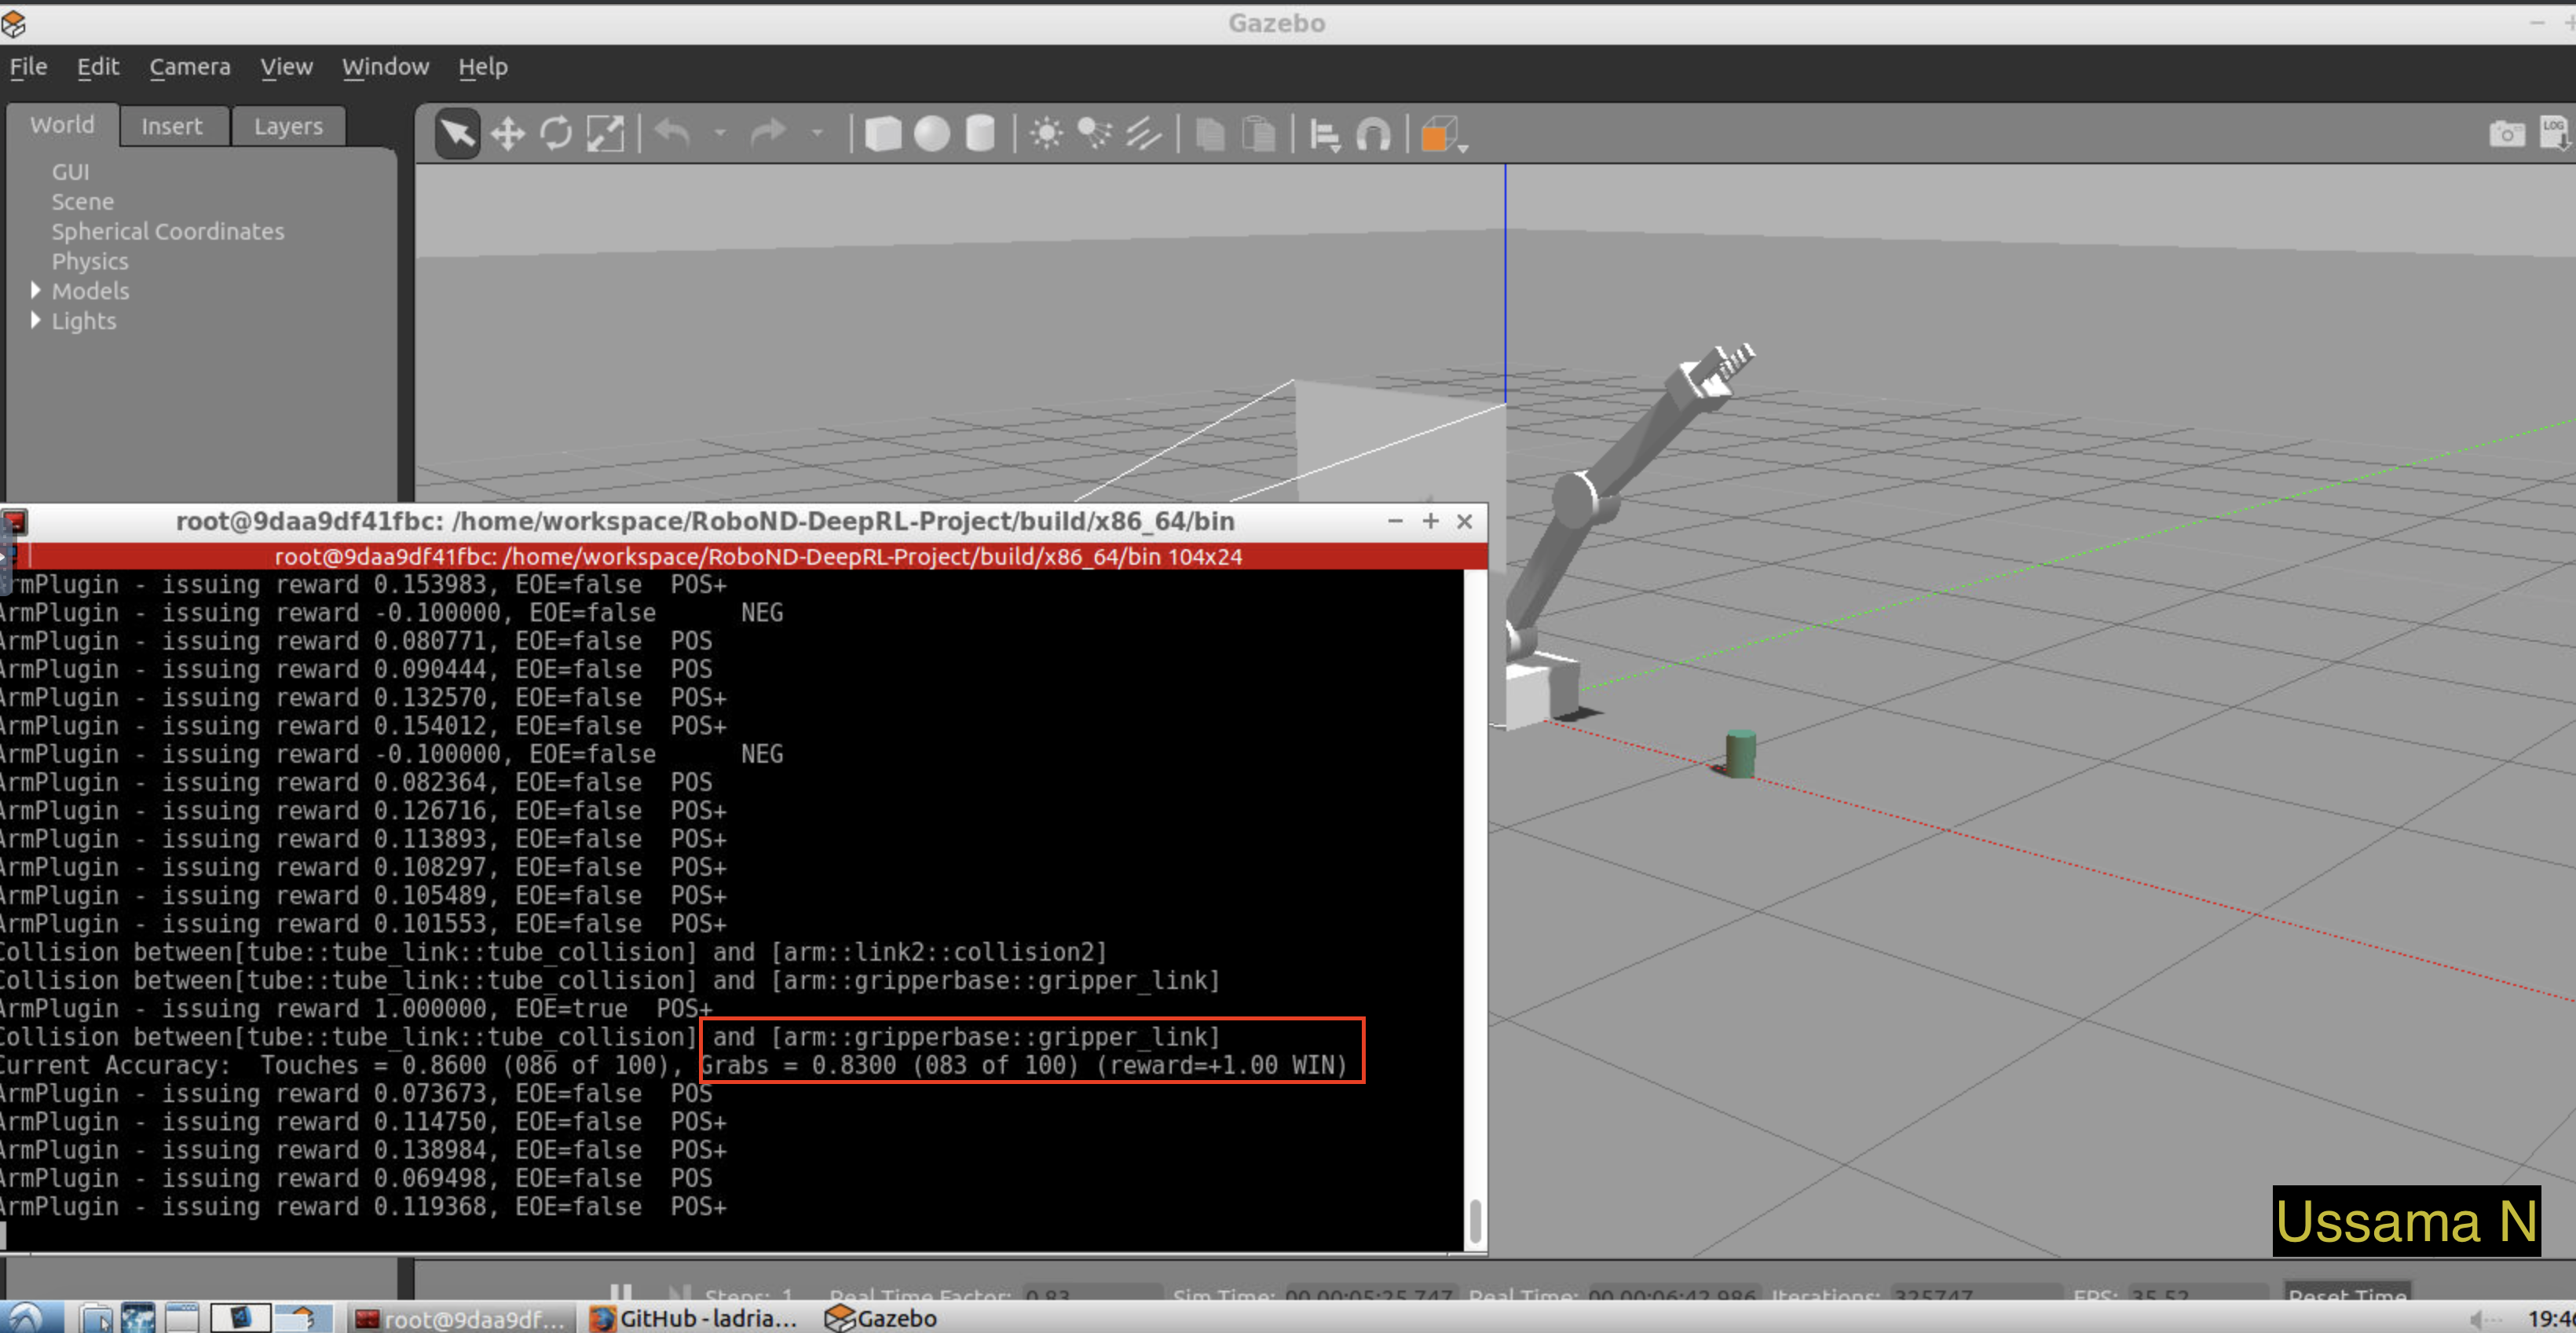
\includegraphics[width=\linewidth]{final-result.png}
      \caption{Best achieved result.}
      \label{fig:robot1}
\end{figure}

%Student should describe and briefly explain the results they achieved for both objectives. The discussion should also include their comments on the DQN agent's performance and if there were any shortcomings.

Doubling the REWARD values for WIN and LOSS from previous tests, had a huge impact on the agent performance. This seems to signal to the agent that the final results is the only that matters.

Some noticeable shortcomings is that the first few iterations greatly decides the final outcome. If the agent was able to touch or grab the object in the beginning, this results in a better chance of the agent achieving the required performance within a 100-150 runs. However, assuming the agent can do more runs then this wouldn't be an issue.

%Student should discuss on what approaches they could take to improve their results.
To improve the results even further, we can let the agent train for longer time such that it will have better chance of discovering the optimal policy. Once the robot learns, we should be able to disable or reduce the amount of randomness in agent and apply the optimal policy and that should give us better results.

Another way to produce better results is to a grid search on the list of parameters.

\end{document}
